\section{The Laser Learning Environment}
\label{sec:LLE}

We introduce here the Laser Learning Environment (LLE), a multi-agent grid world populated by agents of different colours (see \autoref{fig:lvl6-annotated}) and with different types of tiles: floor, start, wall, laser, laser source, gem, and exit tiles. The main objective in LLE is for each agent to reach an exit tile, while additional points can be gathered by collecting gems along the way. The game is cooperative since agents must help each other to pass laser beams:  if an agent's colour doesn't match the colour of a laser beam, this agent dies and the game ends. However, when an agent of matching colour stands in line with a beam, it blocks the laser and allows other agents to reach areas of the map that they could not access by themselves.

LLE comes with 6 different maps (Appendix~\ref{apx:maps}) and can also generate random solvable maps of arbitrary sizes based on multiple parameters (number of agents, number of gems, number of lasers and wall density). Randomly generated maps can also be constrained to some degree of difficulty depending on how many steps of \textit{perfect coordination} (see \autoref{sec:motivations}) are required to complete the level. While future work will address the issue of curriculum learning \citep{parker2022evolving}, in this work, we focus on the configuration visualised in  \autoref{fig:lvl6-annotated}.

\begin{figure}
  \centering
  \scriptsize
  \begin{tikzpicture}
    % Include the image
    \node[anchor=south west, inner sep=0] (image) at (0,0) {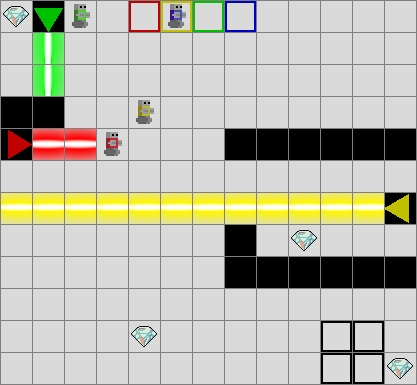
\includegraphics[width=0.4\textwidth]{images/envs/lvl6-block.jpeg}};
    
    % Draw rectangles
     \draw[black,thick] (1.48, 4.08) rectangle ++ (1.6, 0.5) node (start) {};
    \draw[black,thick] (-0.03, 1.82) rectangle ++ (4.58, 0.5) node (laser) {};
    \draw[black,thick] (3.72, -0.03) rectangle ++ (0.84, 0.84) node (exit) {};
    
    % Add annotations
    \node[draw,fill=white, anchor=west] at (3.2, 4.3) {Start tiles};
    \node[draw,fill=white, anchor=west] at (0.5, 1.55) {Yellow laser};
    \node[draw,fill=white, anchor=west, align=center] at (5, 2.1) {Laser\\ source};
    \node[draw,fill=white, anchor=west] at (1.3, 0.2) {Gem};
    \node[draw,fill=white, anchor=west] at (1.9, 3.2) {Yellow agent};
    \node[draw,fill=white, anchor=east] at (3.7, 0.4) {Exit tiles};
  \end{tikzpicture}
  \caption{Level 6 of LLE, which has 4 agents, 3 lasers and 4 gems. Agent red blocks the red laser, making it possible for the other agents to pass to the lower part of the grid world. Additional blocking of the yellow laser is required for them to all pass and reach the exit tiles.}
    \label{fig:lvl6-annotated}
\end{figure}

\subsection{Motivations}
\label{sec:motivations}
As explained in \autoref{sec:environemnts}, there already exist several multi-agent cooperative environments that are suitable for studying various fields of MARL. However, LLE aims at studying a new range of problems. As far as we were able to find the information, LLE introduces new complexities in the study of cooperative problem solving due to a combination of three properties: \textit{perfect coordination}, \textit{interdependence} and \textit{zero incentive dynamics}.

\subsubsection{Perfect coordination}~
is defined as the property of a policy in which agents simultaneously take a specific sequence of actions such that any agent that singlehandedly deviates from this policy in state $s_t$ would directly lead to a penalty in state $s_{t+1}$ and possibly the early termination of the game.

Unlike all the environments presented in \autoref{sec:environemnts}, LLE requires agents to achieve perfect coordination when blocking lasers. Focussing on agents red and yellow in \autoref{fig:lvl6-annotated}, it requires perfect coordination for agent yellow to cross the red laser: if agent yellow goes down and agent red releases the laser, agent yellow would die and the game would terminate with a punishment.
Although Hanabi has the comparable property of directly punishing agents that fail to coordinate, the environment is such that agents play one after the other. For that reason, Hanabi does not require \textit{perfect coordination}.


\subsubsection{Interdependence} \label{sec:prop-interdependence}~ 
%Intuitively, the level of \textit{interdependence} of an environment 
expresses how much a set of agents relies on another set of agents to perform a particular sequence of actions in order to make progress in the collective task.

Interdependence introduces \emph{bottlenecks in the state space} in the steps that require coordination. A high level of interdependence means that from the start state, the end state that maximises the collective expected discounted return is located behind such interdependence bottlenecks. Inversely, a low level of interdependence means that agents can explore most of the state space without relying on each other.

The maps presented in Appendix~\ref{apx:maps} have been designed with increasing levels of interdependence in mind, with level 6 having the highest level of interdependence. In comparison, SMAC, MPE and HLE challenge agents with situations where any agent can explore the state space, sometimes even finish the game, regardless of their teammates' actions.

Overcooked explicitly uses the concept of sub-tasks in the form of recipes that also enclose the reachable state space until the current sub-task is solved. However, agents can most of the time accomplish those sub-tasks by themselves and are therefore not interdependent. Arguably, there is \textit{interdependence} in completely split maps where agents do not have access to every kitchen tool (e.g.: full-divider map) and must pass items over the counter to the other to complete recipes.


\subsubsection{Zero-incentive dynamics} defines the property of an environment in which overcoming bottlenecks in the state space is not rewarded. Intuitively, an environment with zero-incentive dynamics does not reward agents for succeeding at key (cooperative) dynamics. 

As detailed in \autoref{sec:rewards}, blocking lasers in LLE does not provide any reward, and laser-blocking are state space bottlenecks caused by interdependence. Consequently, LLE has zero-incentive dynamics. Overcooked on the other hand provides rewards for finishing recipes and therefore does not have zero-incentive dynamics, even in the full-divider map that does have interdependence. We discuss in \autoref{sec:results} that the combination of interdependence and zero-incentive dynamics makes it difficult for agents to escape regions surrounded by lasers during the training process, which makes LLE a challenging exploration task.

We distinguish zero-incentive dynamics from temporal credit assignment \citep{sutton_1984_credit_assignment}, which is related to the ability of a policy to determine which action takes credit for some later reward, and not a property of the environment.


\subsection{States}
The state of LLE encodes the location of grid-world elements layer by layer as illustrated in \autoref{fig:layered}. These items are namely agents, walls, lasers, laser sources, gems and exits locations. There is one layer per agent and one layer per laser colour. 
This representation has the advantage of being very generic as long as the size of the map and the number of agents remain identical, allowing future work in the field of generalisation and curriculum learning \citep{parker2022evolving}.

\subsection{Actions}
The action space of LLE is discrete and the possible actions are \texttt{NORTH}, \texttt{EAST}, \texttt{SOUTH}, \texttt{WEST} and \texttt{STAY}, which is required for laser-blocking purposes. Actions are identical for all agents.

LLE prevents agents from entering invalid tiles by providing the set of available actions for each agent at each time step. An agent cannot enter walls, move beyond the grid boundaries or enter a tile that is currently occupied by another agent. This prevents multiple types of conflicts that can occur in grid world problems such as edge, following and swapping conflicts \citep{stern_multi-agent_2017_conflicts}.  Additionally, once an agent enters an exit tile, it cannot leave it anymore and the only action allowed is \texttt{STAY}. 

Vertex conflicts -- when two or more agents enter the same tile -- can unfortunately not be prevented with information on action availability. As a result, when agents provoke a vertex conflict by trying to move to the same tile, their actions are replaced by \texttt{STAY}.

\begin{figure}[t]
    \centering
    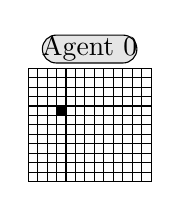
\begin{tikzpicture}[scale=0.12]
        \filldraw[fill=gray!20, rounded corners=5pt] (1.5,15.5) rectangle ++(10,-2.95) node[midway,align=center]{Agent 0};
        \foreach \x in {0,...,12}{
            \foreach \y in {0,...,11}{
                \draw (\x,\y) rectangle ++(1,1);
            }
        }
        \fill[black] (3,7) rectangle ++(1, 1);
    \end{tikzpicture} 
    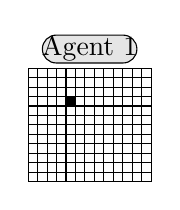
\begin{tikzpicture}[scale=0.12]
        \filldraw[fill=gray!20, rounded corners=5pt] (1.5,15.5) rectangle ++(10,-2.95) node[midway,align=center]{Agent 1};
        \foreach \x in {0,...,12}{
            \foreach \y in {0,...,11}{
                \draw (\x,\y) rectangle ++(1,1);
            }
        }
        \fill[black] (4,8) rectangle ++(1, 1);
    \end{tikzpicture}
    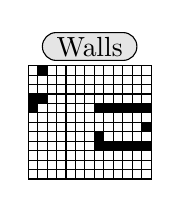
\begin{tikzpicture}[scale=0.12]
        \filldraw[fill=gray!20, rounded corners=5pt] (1.5,15.5) rectangle ++(10,-2.95) node[midway,align=center]{Walls};
        \foreach \x in {0,...,12}{
            \foreach \y in {0,...,11}{
                \draw (\x,\y) rectangle ++(1,1);
            }
        }
        \fill[black] (0,7) rectangle ++(1, 1);
        \fill[black] (0,8) rectangle ++(1, 1);
        \fill[black] (1,8) rectangle ++(1, 1);
        \fill[black] (1,11) rectangle ++(1, 1);

        \foreach \x in {7,...,12}{
            \fill[black] (\x,7) rectangle ++(1, 1);
        }

        \foreach \x in {7,...,12}{
            \fill[black] (\x,3) rectangle ++(1, 1);
        }
        \fill[black] (7,4) rectangle ++(1, 1);
        \fill[black] (12,5) rectangle ++(1, 1);
    \end{tikzpicture}
    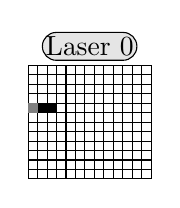
\begin{tikzpicture}[scale=0.12]
        \filldraw[fill=gray!20, rounded corners=5pt] (1.5,15.5) rectangle ++(10,-2.95) node[midway,align=center]{Laser 0};
        \foreach \x in {0,...,12}{
            \foreach \y in {0,...,11}{
                \draw (\x,\y) rectangle ++(1,1);
            }
        }
        \fill[gray] (0,7) rectangle ++(1, 1);
        \fill[black] (1,7) rectangle ++(1, 1);
        \fill[black] (2,7) rectangle ++(1, 1);
    \end{tikzpicture}
    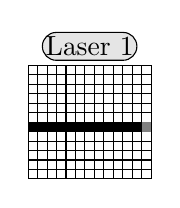
\begin{tikzpicture}[scale=0.12]
        \filldraw[fill=gray!20, rounded corners=5pt] (1.5,15.5) rectangle ++(10,-2.95) node[midway,align=center]{Laser 1};
        \foreach \x in {0,...,12}{
            \foreach \y in {0,...,11}{
                \draw (\x,\y) rectangle ++(1,1);
            }
        }
        \foreach \x in {0,...,11}{
            \fill[black] (\x,5) rectangle ++(1, 1);
        }
        \fill[gray] (12,5) rectangle ++(1, 1);
    \end{tikzpicture}
    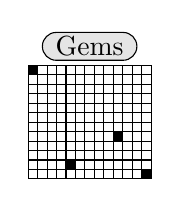
\begin{tikzpicture}[scale=0.12]
        \filldraw[fill=gray!20, rounded corners=5pt] (1.5,15.5) rectangle ++(10,-2.95) node[midway,align=center]{Gems};
        \foreach \x in {0,...,12}{
            \foreach \y in {0,...,11}{
                \draw (\x,\y) rectangle ++(1,1);
            }
        }
        \fill[black] (0,11) rectangle ++(1, 1);
        \fill[black] (12,0) rectangle ++(1, 1);
        \fill[black] (4,1) rectangle ++(1, 1);
        \fill[black] (9,4) rectangle ++(1, 1);
    \end{tikzpicture}
    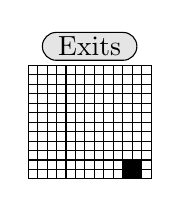
\begin{tikzpicture}[scale=0.12]
        \filldraw[fill=gray!20, rounded corners=5pt] (1.5,15.5) rectangle ++(10,-2.95) node[midway,align=center]{Exits};
        \foreach \x in {0,...,12}{
            \foreach \y in {0,...,11}{
                \draw (\x,\y) rectangle ++(1,1);
            }
        }
        \foreach \x in {10,...,11}{
            \foreach \y in {0,...,1}{
                \fill[black] (\x,\y) rectangle ++(1, 1);
            }
        }
    \end{tikzpicture}

    \caption{Representation of the state shown in \autoref{fig:lvl6-annotated}. The layers ``Agent 2'', ``Agent 3'', ``Laser 2'' and ``Laser 3'' were omitted for the sake of conciseness. Each layer encodes the location of a specific type of object of the grid world (walls, agents' locations, \dots). White squares represent $0$s, black squares are $1$s and grey squares are $-1$.}
    \label{fig:layered}
\end{figure}

\subsection{Rewards}
\label{sec:rewards}
The reward function of LLE has a single scalar output as the team reward, which is the result of the joint action of the agents at a given time step. Collecting a gem or entering an exit tile provides a collective reward of $+1$. Finishing the game, i.e. when all agents are on an exit tile, also provides an additional reward of $+1$. However, if any agent dies at a time step, the episode ends and the reward is set to $-1$ times the number of agents that have died.


\subsection{Metrics}
\label{sec:metrics}
Two metrics are used here to evaluate the performance of the LLE agents: the score and the exit rate.

\subsubsection{Score}
The score refers to the undiscounted sum of rewards throughout an episode. This is metric is close to the one the agents are trained to maximise, i.e. the \textit{discounted} sum of rewards over the course of an episode, but does not give insight on the time taken to achieve the task. The maximal score of an LLE environment can be calculated as follows: given a map with $n$ agents and $g$ gems, we can compute the maximum score as $\text{maximum score} = n + g + 1$.


\subsubsection{Exit rate}
The exit rate is defined as the proportion of agents that reach an exit tile at the end of an episode. Since the objective in every LLE is to exit the level, this metric gives an estimation of how close agents are to the objective. An exit rate of $1$ means that all agents have successfully exited the level.\\

The combination of those two metrics gives insight into the agents' behaviour. As long as the exit rate is below 1, it means that the agents are not able to finish the level. If the exit rate is 1, then analysing the score allows us to know if agents have collected all the gems.



\subsection{Implementation}
LLE is implemented in Rust which makes it an extremely fast environment. LLE comes with a strongly type hinted Python interface for seamless integration with common MARL libraries and is extensively tested in both Python and Rust.